\section{Policy Gradient Methods}
So far the methods discussed select actions based on estimated (state-)action­ values, however this is not the only option. Instead of learning the value estimates and deriving a policy out of the resulting value functions, it is also possible to directly learn a \emph{parametrized policy} which can choose actions without having to consult a value function.

Policy gradient methods are a class of learning methods that learn the policy parameters, $\nd{\theta}$, based on the gradient of some performance measure, $J\left(\nd{\theta}\right)$, with respect to the policy parameters. These methods try to maximize the performance, so the updates approximate gradient accent in $J$. 

\begin{equation}
  \nd{\theta_{t+1}} = \nd{\theta_t} + \alpha \cdot \widehat{\nabla J\left(\nd{\theta_t}\right)}
  \label{eq:stochastic_gradient_ascent}
\end{equation}

where $\alpha$ is a positive step-size parameter and $\widehat{\nabla J\left(\nd{\theta_t}\right)}$ is a stochastic estimate who's expectation is the gradient of the performance measure with respect to $\nd{\theta_t}$.

An advantage of using policy gradient over \eps-greedy action selection is that the approximate policy can approach a deterministic policy if the optimal policy is deterministic, whereas \eps-greedy action selection will always have an \eps \ probability of selecting a random action.

Similarly if the optimal policy is stochastic or in cases where multiple actions have similar values, then policy gradient methods are able to converge towards stochastic policies who's probability distribution approximate the distribution of the optimal policy. In contrast action-value methods are unable to find optimal stochastic policies.

In problems with significant function approximation, the best policy may be stochastic even for deterministic problems. With imperfect information the optimal policy may be to perform two or more different actions with specific probabilities, for example when bluffing in Poker.

This is specially helpful for continuos state and action spaces. Since, as discussed in Section~\ref{sec:approximate_solutions}, for these kind of systems it is usually not practical to store, process and learn policy and value functions based on tables. Instead these functions are usually approximated.
 
\subsection{Policy parameterization}
In policy gradient methods the policy may be parametrized in any way so long as the policy function, $\pi\left(a|s,\ \nd{\theta}\right )$, is differentiable with respect to the policy parameters, $\nd{\theta}$. 

A method of parameterization in case of discreet and small action spaces is to form parametrized numerical preferences $h(s, a, \nd{\theta}) \in \mathbb{R}$ for each state-action pair. The actions with the highest preference can then be given the highest probability of being selected by, for example, using an exponential softmax distribution,

\begin{equation}
  \pi\left(a|s, \nd{\theta}\right)=\frac{\exp(h(s, a, \nd{\theta}))}{\sum_b\exp(h(s, b, \nd{\theta}))}
\end{equation}

The denominator is needed such that the probabilities in each state sum to one, thus allowing the preference to be parametrized using any function, whether it is a table, a linear function using feature vectors or a deep neural network.

For problems with large or continuos action spaces it may be better to learn the statistics of the probability distribution instead of the preference of each individual action. For example, the actions may be chosen using a normal (Gaussian) distribution. In this case the mean, $\mu$, and standard deviation, $\sigma$, of the distribution may be parametrized using any function approximation method, with the only limitation being that the function for the standard deviation must always be positive.

\begin{equation}
  \pi\left(a|s, \nd{\theta}\right)=\frac{1}{\sigma(s, \nd{\theta})\sqrt{2\pi}}\exp\left(-\frac{(a-\mu(s, \theta))^2}{2\sigma(s, \theta)^2}\right)
\end{equation}

\subsection{Policy gradient theorem}

The goal with \gls{mdp} problems is to find a policy which maximizes the sum of rewards the agent receives. The value function approximates an expectation of the sum of rewards, thus the perform measure, $J\left(\nd{\theta}\right)$, can be assumed as being approximately equal to the true value function under current policy $\pi_\theta$.

\begin{equation}
  J\left(\nd{\theta}\right) \doteq v_{\pi_\theta}\left(s\right)
\end{equation}

The problem with finding a change in the policy parameters that ensures improvement is that the performance depends on both the action selection and the distribution of states. At a given state, estimating the effect on the actions, and thus the reward, is relatively straightforward. However the effect of the policy on the state distribution depends on effects from the environment which are typically unknown.

Fortunately, the \emph{policy gradient theorem} provides an analytical expression that is proportional to the gradient of the performance with respect to the policy parameters, which doesn't involve the derivative of the state distribution\cite{sutton2018reinforcement}.

\begin{equation}
  \nabla J\left(\nd{\theta}\right) \propto \sum_s \mu \left(s\right) \sum_a q_\pi\left(s, a\right) \nabla_\theta \pi\left(a|s, \nd{\theta}\right)
  \label{eq:pgt}
\end{equation}

\subsection{REINFORCE}
Recall from Equation~\ref{eq:stochastic_gradient_ascent} the overall strategy for policy gradient methods requires an estimate of the gradient of the performance measure with respect to the policy parameters. This estimate only needs to be proportional to the real gradient, since any constant of proportionality can be absorbed by the step size $\alpha$, which is otherwise arbitrary. The policy gradient theorem (Equation~\ref{eq:pgt}) gives an expression for such an estimate.

The right-hand side of the policy gradient theorem is a sum over the states weighted by how often the states occur under the target policy $\pi$. If $\pi$ is followed, then the states will be encountered in these proportions. Thus,

\begin{align}
  \nabla J\left(\nd{\theta}\right) &\propto \sum_s \mu \left(s\right) \sum_a q_\pi\left(s, a\right) \nabla_\theta \pi\left(a|s, \nd{\theta}\right)\\
  &= \mathbb{E}_\pi\left[\sum_a q_\pi\left(S_t, a\right) \nabla_\theta \pi\left(a|S_t, \nd{\theta}\right)\right]
\end{align}

The remaining part of the expectation is a sum over the actions. If each term was weighted by the probability of selecting the actions, that is by, $\pi\left(a|S_t,\theta\right)$, then it is possible to replace $a$ by the sample action $A_t$. This can be done by multiplying and dividing by this probability.

\begin{align}
  \nabla J\left(\nd{\theta}\right)&= \mathbb{E}_\pi\left[\sum_a \pi\left(a|S_t,\theta\right)q_\pi\left(S_t, a\right) \frac{\nabla_\theta \pi\left(a|S_t, \nd{\theta}\right)}{\pi\left(a|S_t,\theta\right)}\right]\\
  &=\mathbb{E}_\pi\left[q_\pi\left(S_t, A_t\right) \frac{\nabla_\theta \pi\left(A_t|S_t, \nd{\theta}\right)}{\pi\left(A_t|S_t,\theta\right)}\right]&\text{(replacing $a$ by sample $A_t \sim \pi$)}\\
  &=\mathbb{E}_\pi\left[G_t \frac{\nabla_\theta \pi\left(A_t|S_t, \nd{\theta}\right)}{\pi\left(A_t|S_t,\theta\right)}\right]&\text{(Because $\mathbb{E}_\pi\left[G_t|S_t, A_t\right]=q_\pi\left(S_t, A_t\right)$, Equation~\ref{eq:value_state_action_pair})}
\end{align}

Substituting this expression into Equation~\ref{eq:stochastic_gradient_ascent} yields the update rule,

\begin{equation}
  \nd{\theta_{t+1}} = \nd{\theta_t} + \alpha G_t \frac{\nabla_\theta \pi\left(A_t|S_t, \nd{\theta}\right)}{\pi\left(A_t|S_t,\theta\right)}
  \label{eq:reinforce_1}
\end{equation}

This is the REINFORCE algorithm. Note that REINFORCE uses the complete return from $t$ until the end of the episode. In this sense REINFORCE is a Monte Carlo algorithm and is thus only well defined for episodic problems.

Each update is proportional to the product of the return, $G_t$, and a vector in the direction that most increases the probability of taking $A_t$ on future visits to $S_t$. This vector is the \emph{eligibility vector}. The eligibility vector is usually written in the more compact form $\nabla_\theta \ln \pi\left(A_t|S_t, \nd{\theta}\right)$, using $\nabla \ln x=\frac{\nabla x}{x}$. Thus the REINFORCE algorithm may also be written as,

\begin{equation}
  \nd{\theta_{t+1}} = \nd{\theta_t} + \alpha G_t \nabla_\theta \ln \pi\left(A_t|S_t, \nd{\theta}\right)
  \label{eq:reinforce_2}
\end{equation}

\subsection{REINFORCE with baseline}
The policy gradient theorem can be generalized by including a comparison of the action value to an arbitrary baseline $b(s)$. 

\begin{equation}
  \nabla J\left(\nd{\theta}\right) \propto \sum_s \mu \left(s\right) \sum_a \left(q_\pi\left(s, a\right) - b(s)\right) \nabla_\theta \pi\left(a|s, \nd{\theta}\right)
  \label{eq:pgt_b}
\end{equation}

This baseline can be any function, even a random variable, as long as it does not vary with the action\cite{sutton2018reinforcement}. Following a similar procedure as in the previous section yields the following update rule for REINFORCE with baseline,

\begin{equation}
  \nd{\theta_{t+1}} = \nd{\theta_t} + \alpha \left(G_t - b(S_t)\right) \frac{\nabla_\theta \pi\left(A_t|S_t, \nd{\theta}\right)}{\pi\left(A_t|S_t,\theta\right)}
  \label{eq:reinforce_baseline}
\end{equation}

The baseline leaves the expected value of the update unchanged, however it can have a large effect on its variance and thus the learning rate. An appropriate choice for the baseline is an estimate of the state-value function $\hat{v}\left(S_t\right)$\cite{sutton2018reinforcement}. In this case, the term with the expected return and baseline value function is known as the expected advantage function.

\begin{equation}
  A_t=G_t-\hat{v}(S_t)
\end{equation}

Since REINFORCE is a Monte Carlo method for learning the policy parameters $\theta$, it seems appropriate to use the similar \acrfull{sgd} function approximation learning method shown in Section~\ref{sec:stochastic_gradient_decent_methods} to learn the value function with weights $\nd{w}$.

\subsection{Actor-Critic}
Methods that learn both the policy and value functions are called \emph{actor-critic} methods, where the actor refers to the learned policy, and the critic to the learned value function. However REINFORCE with baseline is not considered an actor-critic method because the state-value function is only used as a baseline and not a critic. That is, it is not used for \emph{bootstrapping}, the process of updating the value estimate of a state using the estimated values of future states, such as with the \acrfull{td} methods found in Section~\ref{sec:temporal_difference}.

Consider the one-step actor-critic methods. These methods replace the complete return used in REINFORCE with baseline with the one-step return. Expanding these methods to include $n$-step bootstrapping is then straightforward.

\begin{align}
  \nd{\theta_{t+1}} &= \nd{\theta_t} + \alpha \left(G_{t:t+1} - \hat{v}\left(S_t, \nd{w}\right)\right) \frac{\nabla_\theta \pi\left(A_t|S_t, \nd{\theta}\right)}{\pi\left(A_t|S_t,\theta\right)}\\
  &= \nd{\theta_t} + \alpha \left(R_{t+1} + \gamma V_t(S_{t+1}) - \hat{v}\left(S_t, \nd{w}\right)\right) \frac{\nabla_\theta \pi\left(A_t|S_t, \nd{\theta}\right)}{\pi\left(A_t|S_t,\theta\right)}\\
  &= \nd{\theta_t} + \alpha \delta_t \frac{\nabla_\theta \pi\left(A_t|S_t, \nd{\theta}\right)}{\pi\left(A_t|S_t,\theta\right)}
  \label{eq:actor-critic_1}
\end{align}



\subsection{PPO}
\label{sec:ppo_algo}
A limitation of standard policy gradient methods is that it is hard to choose step sizes when updating the policy. This is in part because a bad update step is quite damaging since it may reduce the visitation distribution around the state. Stepping to far results in a bad policy, which leads to new data being collected under the bad policy, which can cause performance collapse. Another issue with standard policy gradient methods is that these methods have low sample efficiency, only one gradient step is performed per environment sample\cite{schulman2017proximal, schulman2015trust}.

So, how can the biggest improvement step on the policy be taken without over stepping and causing performance collapse? This is the question that methods such as \acrfull{trpo}, and \acrfull{ppo} seek to answer.

% To better visualize the main issue, imagine an agent is climbing a mountain with the goal being to reach top. However somewhere along its path it must cross a narrow pass with cliffs. If the agent takes short steps it will take too long to reach the top. If the steps are too long it may fall off the cliff and land in a bad state with low rewards, which will lead to a locally bad policy. 

% Using the trust region method a maximum change in policy is chosen. Then the optimal point within the trust region is selected and the search continuos from there. But how is the size of this thrust region chosen? 

In \acrshort{trpo} a surrogate objective function is maximized. This function is an approximation of the expected advantage function of the current or new policy. It is the expected advantage from the old policy being used when the sample was taken and then calibrated using the probability ratio between the new and old policies. This approximation becomes less accurate, as the two policies deviate from each other.

This objective function is then constrained by the KL-divergence of the new and old policies. The KL-divergence function measures the difference between two probability distributions. This problem is then solved using the conjugate gradient algorithm after making a linear approximation of the objective function and a quadratic approximation of the constraint \cite{schulman2015trust}.

\begin{equation}
  \begin{aligned}
  & \underset{\theta}{\text{maximize}}
  & & \mathbb{E_t} \left[\frac{\pi_\theta(a_t | s_t)}{\pi_{\theta_{old}}(a_t | s_t)} A_t\right] \\
  & \text{subject to}
  & & \mathbb{E_t}\left[\overline{KL}\left[ \pi_{\theta_{old}}(\cdot | s_t), \pi_\theta(
    \cdot | s_t) \right]\right] \leq \delta
  \end{aligned}
  \label{eq:trpo_constraint}
  \end{equation}
  x sc
The theory justifying \acrshort{trpo} actually suggests using a penalty instead of a constraint as shown in Equation~\ref{eq:trpo_penalty}. In this case the objective function computes the maximum KL-divergence over the states and subtracts it from the expected advantage estimate,forming a lower or pessimistic bound on the performance of the new policy, $\pi$. This lower bound function can then be used to optimize the policy for maximum rewards using the \acrfull{mm} algorithm shown in Figure~\ref{fig:mma}. \acrshort{mm} works by iteratively maximizing a lower bound function which locally approximates the target function.

\begin{equation}
  \begin{aligned}
  & \underset{\theta}{\text{maximize}}
  & & \mathbb{E_t} \left[
    \frac{\pi_\theta(a_t | s_t)}{\pi_{\theta_{old}}(a_t | s_t)} A_t
    - \beta\ \overline{KL}\left[ \pi_{\theta_{old}}(\cdot | s_t), \pi_\theta(\cdot | s_t) \right]
  \right]   
  \end{aligned}
  \label{eq:trpo_penalty}
  \end{equation}

\begin{figure}[h!]			
	\centering
	

\tikzset{every picture/.style={line width=0.75pt}} %set default line width to 0.75pt        

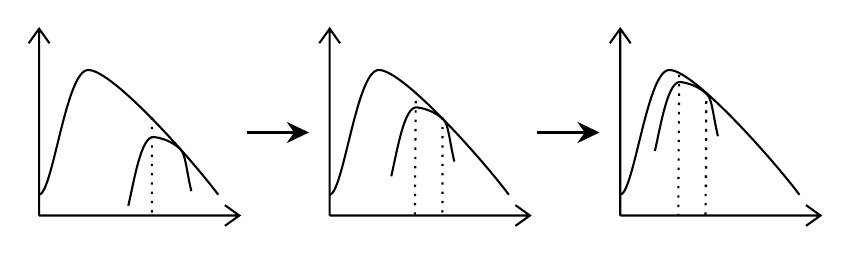
\begin{tikzpicture}[x=0.75pt,y=0.75pt,yscale=-1,xscale=1]
%uncomment if require: \path (0,300); %set diagram left start at 0, and has height of 300

%Shape: Axis 2D [id:dp4587948033811651] 
\draw  (10,90) -- (106.5,90)(10,0) -- (10,90) -- cycle (99.5,85) -- (106.5,90) -- (99.5,95) (5,7) -- (10,0) -- (15,7)  ;
%Curve Lines [id:da18911843907310866] 
\draw    (10,80) .. controls (16.46,79.46) and (22.66,22.56) .. (32.86,20) .. controls (43.05,17.44) and (82.7,61.82) .. (96.34,80) ;
%Curve Lines [id:da6036550847648126] 
\draw    (52.97,85.37) .. controls (55.91,72.47) and (59.27,51.37) .. (65.36,52.17) .. controls (71.46,52.97) and (76,55.9) .. (78.26,58.27) .. controls (80.52,60.64) and (80.8,67.09) .. (83.34,78.27) ;
%Straight Lines [id:da8578471473751457] 
\draw  [dash pattern={on 0.84pt off 2.51pt}]  (64.38,42.77) -- (64.34,90) ;

%Shape: Axis 2D [id:dp6574954797817647] 
\draw  (150,90) -- (246.5,90)(150,0) -- (150,90) -- cycle (239.5,85) -- (246.5,90) -- (239.5,95) (145,7) -- (150,0) -- (155,7)  ;
%Curve Lines [id:da25965914680457214] 
\draw    (150,80) .. controls (156.46,79.46) and (162.66,22.56) .. (172.86,20) .. controls (183.05,17.44) and (222.7,61.82) .. (236.34,80) ;
%Straight Lines [id:da6096091820649563] 
\draw  [dash pattern={on 0.84pt off 2.51pt}]  (204.38,42.77) -- (204.34,90) ;
%Curve Lines [id:da026999812862924077] 
\draw    (179.68,71.09) .. controls (182.63,58.19) and (185.98,37.09) .. (192.07,37.89) .. controls (198.17,38.69) and (202.71,41.61) .. (204.98,43.99) .. controls (207.24,46.36) and (207.51,52.81) .. (210.05,63.99) ;
%Straight Lines [id:da16767819972771236] 
\draw  [dash pattern={on 0.84pt off 2.51pt}]  (191.5,30.43) -- (191.07,90) ;

%Shape: Axis 2D [id:dp0015559830363194305] 
\draw  (290,90) -- (386.5,90)(290,0) -- (290,90) -- cycle (379.5,85) -- (386.5,90) -- (379.5,95) (285,7) -- (290,0) -- (295,7)  ;
%Curve Lines [id:da2098671626464952] 
\draw    (290,80) .. controls (296.46,79.46) and (302.66,22.56) .. (312.86,20) .. controls (323.05,17.44) and (362.7,61.82) .. (376.34,80) ;
%Straight Lines [id:da74842077971829] 
\draw  [dash pattern={on 0.84pt off 2.51pt}]  (331.38,30.57) -- (331.34,77.8) ;
%Curve Lines [id:da9364855762625719] 
\draw    (306.68,58.89) .. controls (309.63,45.99) and (312.98,24.89) .. (319.07,25.69) .. controls (325.17,26.49) and (329.71,29.41) .. (331.98,31.79) .. controls (334.24,34.16) and (334.51,40.61) .. (337.05,51.79) ;
%Straight Lines [id:da24011628952109132] 
\draw  [dash pattern={on 0.84pt off 2.51pt}]  (331.5,30.43) -- (331.14,80.6) -- (331.07,90) ;
%Straight Lines [id:da47850878943087705] 
\draw  [dash pattern={on 0.84pt off 2.51pt}]  (318.41,22.25) -- (318.05,72.42) -- (317.97,90.05) ;

%Straight Lines [id:da9966472179405139] 
\draw    (110,50) -- (137,50) ;
\draw [shift={(140,50)}, rotate = 180] [fill={rgb, 255:red, 0; green, 0; blue, 0 }  ][line width=0.08]  [draw opacity=0] (10.72,-5.15) -- (0,0) -- (10.72,5.15) -- (7.12,0) -- cycle    ;
%Straight Lines [id:da45480919688203447] 
\draw    (250,50) -- (277,50) ;
\draw [shift={(280,50)}, rotate = 180] [fill={rgb, 255:red, 0; green, 0; blue, 0 }  ][line width=0.08]  [draw opacity=0] (10.72,-5.15) -- (0,0) -- (10.72,5.15) -- (7.12,0) -- cycle    ;




\end{tikzpicture}
			
	\caption{Minorize-Maximization algorithm}
	\label{fig:mma}
\end{figure}

The reason \acrshort{trpo} uses a hard constraint instead of the penalty is because it is difficult to choose a value for $\beta$ that works well between problems or even within the same problem. However \acrshort{ppo} provides new alternate surrogate objective functions that work around this issue. Despite \acrshort{ppo} not being as good as \acrshort{trpo} in determining an appropriate size for the trust region, it is much simpler to implement and less computationally intensive. Benchmarks show that \acrshort{ppo} is able to perform as good as or even better than other state-of-the-art methods\cite{schulman2017proximal}. 

There are two variants of \acrshort{ppo}. \acrshort{ppo} with adaptive KL penalty and \acrshort{ppo} with clipped objective. This thesis only uses \acrshort{ppo} with clipped objective, thus the first variant is left out.

Let $r_t(\nd\theta)$ be the probability ratio $r_t(\nd\theta)=\frac{\pi_\theta(a_t | s_t)}{\pi_{\theta_{old}}(a_t | s_t)}$. Then the policy surrogate objective function proposed by \acrshort{ppo} is as follows.

\begin{equation}
  L_t^{CLIP}(\nd{\theta}) = \mathbb{E_t} \left[\min(
    r_t(\nd\theta)A_t,
    \text{clip}(r_t(\nd\theta), 1-\epsilon, 1+\epsilon)A_t
  )\right]
\end{equation}

Where \eps\ is a hyperparameter, in the original paper the value of $\epsilon=0.2$ was chosen based on benchmarks\cite{schulman2017proximal}. The first term inside the $\min(\dots)$ is the same as the surrogate objective function used in \acrshort{trpo} (Equation~\ref{eq:trpo_constraint}). The second term $\text{clip}(r_t(\nd\theta), 1-\epsilon, 1+\epsilon)A_t$ modifies the surrogate objective by clipping the probability ratio, thus removing the incentive for moving $r_t$ outside of the interval $\left[1-\epsilon, 1+\epsilon\right]$

If a neural network architecture that shares parameters between the policy and value functions is being used, then a loss function that combines the policy surrogate objective function and a value function error term must be used. An entropy bonus may also be added to encourage exploration. Combining these terms results in the following objective function\cite{schulman2017proximal}.

\begin{equation}
  L_t^{CLIP+VF+S}(\nd{\theta}) = \mathbb{E_t} \left[ 
    L_t^{CLIP}(\nd{\theta}) +
    c_1L_t^{VF}(\nd{\theta}) +
    c_2S[\pi_\theta](s_t) 
    \right]
\end{equation}

Here are $c_1$ and $c_2$ coefficients, $S$ the entropy bonus and $L_t^{VF}$ is the squared-error loss of the value function estimate. This objective function can then be optimized on each iteration using \acrshort{sgd} or Adam. This allows each environment sample to be used for multiple policy updates, thus resulting in a better sample efficiency than standard gradient decent methods.




